\documentclass[a4paper,bcor=0mm,9pt,parskip=full,twoside]{tubsartcl}
\usepackage[utf8]{inputenc}

\usepackage[balancingshow]{multicol}

\usepackage{lipsum}

\begin{document}


\begin{gaussbox}[bgcolor=tuGreenLight]{1}{1}{6}{8}
© Technische\\
Universität Braunschweig\\
Name des Instituts oder der zentralen Einrichtung\\
Musterstr. 4 – 5\\
38106 Braunschweig\\
Telefon +49 531 391-0000\\
Telefax +49 531 391-0000\\
institut@tu-braunschweig.de\\
www.tu-braunschweig.de
\end{gaussbox}
~\clearpage

% \begin{gaussbox}[bgcolor=tubsOrange20,fgcolor=tuOrange]{1}{1}{6}{8}
\headline{\color{tuOrange}Headline Sans 45pt.\\
Dunt acilluptat Putat-\\
quamacone sit}
\vspace*{2.5cm}
\setlength\postmulticols{0mm}
\begin{minipage}{\textwidth}
\begin{multicols}{2}
\lipsum[2]\par~\par\columnbreak
\lipsum[4]\par
\end{multicols}
\end{minipage}
\vspace*{0.5cm}
\begin{multicols*}{2}
\bfseries\sffamily Diagrammüberschrif in Nexus Sans Bold\par
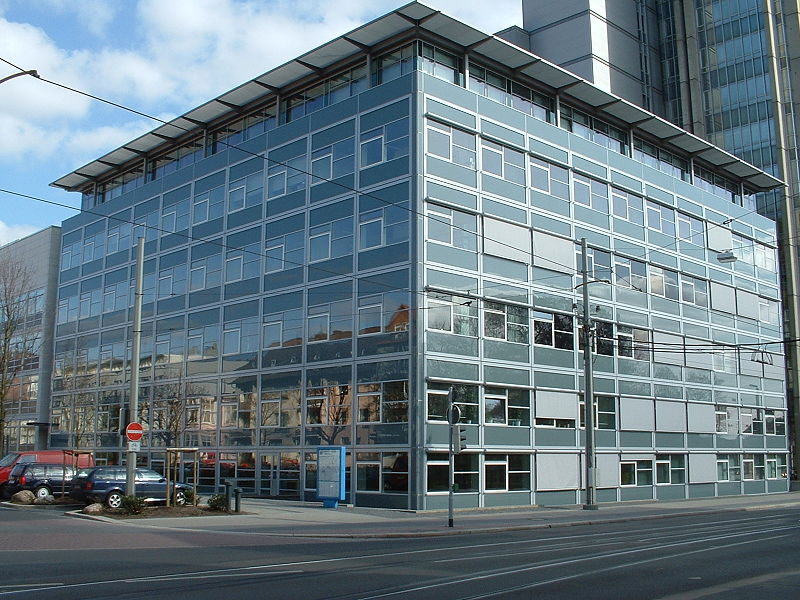
\includegraphics[width=\linewidth]{infozentrum}
\end{multicols*}
\clearpage

\bglayout[pages=single]{
  \showtubslogo
  \bgsegment[bgcolor=tuOrange]{2}
  \bgsegment[bgcolor=tuOrange80]{4}
  \bgsegment[bgcolor=tuOrange60]{2}
}

\begin{gaussbox}[logosep]{1}{1}{2}{8}
\large
\lipsum[4]
\end{gaussbox}
\begin{gaussbox}[c]{3}{1}{2}{8}
\large
\lipsum[2]
\end{gaussbox}
\begin{gaussbox}[b]{5}{1}{2}{8}
\large
\lipsum[2]
\end{gaussbox}
~\clearpage

\begin{gaussbox}{1}{1}{5}{1}
{\LARGE\sffamily\bfseries\raggedright Atueriliquat volore feui eui bla
aliquissit atie vulla feum vent
adipit wis acipsus cipit, si.\par}
\end{gaussbox}
\begin{gaussbox}[frame=fbox]{2}{2}{5}{1}
\usekomafont{institute}\mdseries
Verostrud eugiamet vel dolor ilismolummy nosto conse mod tie
faccum vullan hendit landipisim veraessim vel ullutim irilluptat volor
sequamc onsectet, qui eu facilit alit, vel utpat lore ming eratie dolor
inci bla feuguero odionsed eniamco veliquat lam Dignit atetum verit
ex erit velisci llandigna famur.
\end{gaussbox}
\begin{gaussbox}[c,bgcolor=tuGray20]{1}{3}{5}{6}
\lipsum[2]\par
\lipsum[2]\par
\end{gaussbox}
\clearpage~\clearpage

\begin{gaussbox}[bgcolor=tubsGray20,outerpadding=hnone,innerpadding=columnsep]{1}{1}{2}{1}
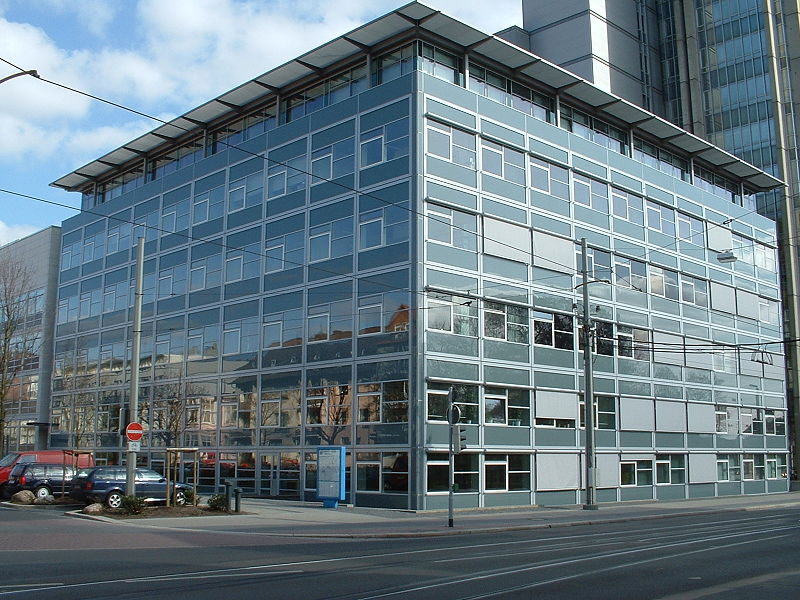
\includegraphics{infozentrum}
\end{gaussbox}
\begin{gaussbox}[bgcolor=tubsGray20,logosep,imagefit=scaled]{3}{1}{2}{1}
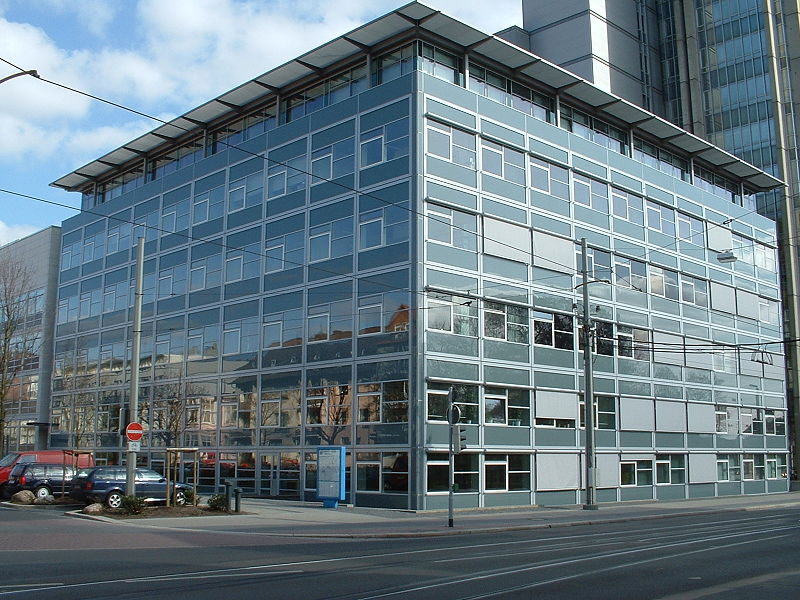
\includegraphics{infozentrum}
\end{gaussbox}
\begin{gaussbox}[bgcolor=tubsBlue20,outerpadding=vnone]{5}{1}{2}{1}
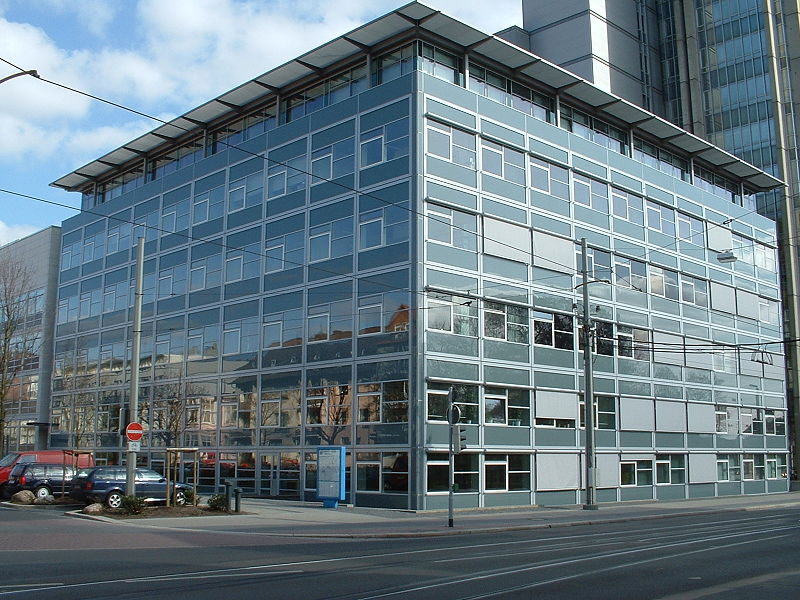
\includegraphics{infozentrum}
\end{gaussbox}
%
\begin{gaussbox}[bgcolor=tubsGray20,innerpadding=columnsep]{1}{2}{2}{1}
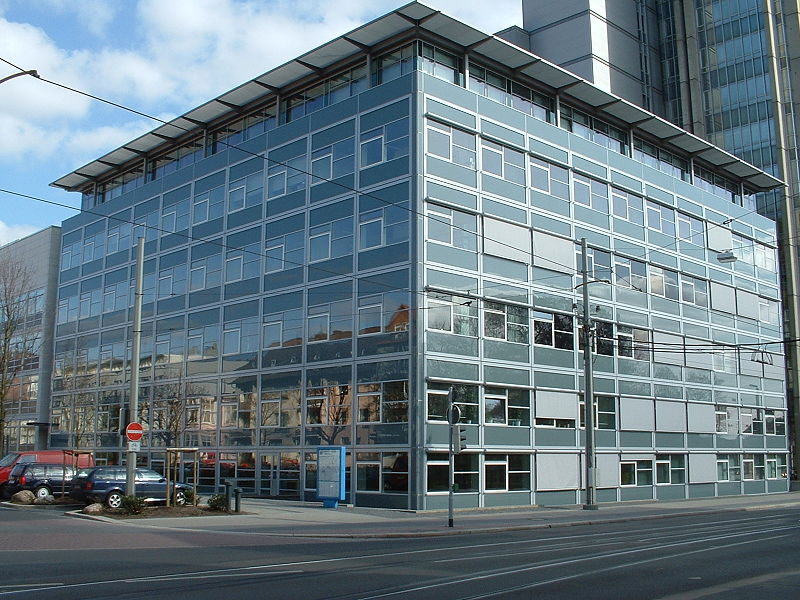
\includegraphics{infozentrum}
\end{gaussbox}
\begin{gaussbox}[bgcolor=tubsGray20,innerpadding=default]{3}{2}{2}{1}
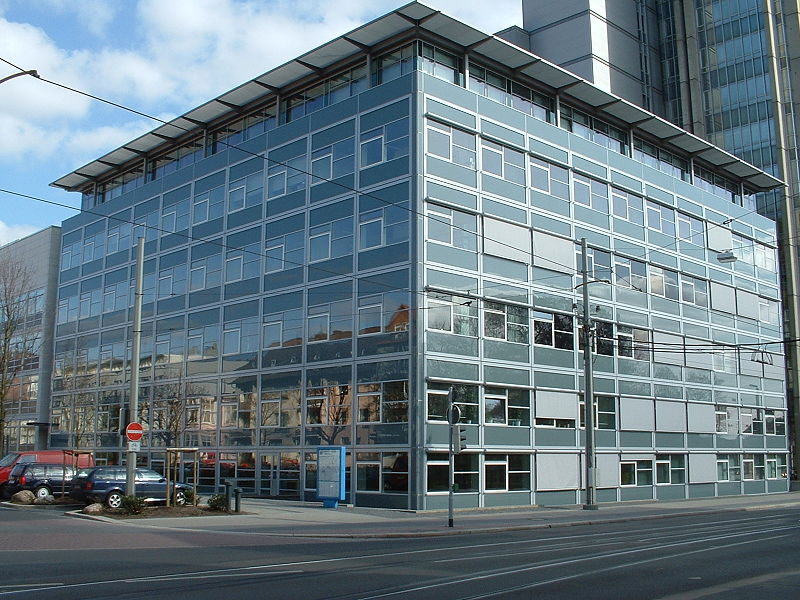
\includegraphics{infozentrum}
\end{gaussbox}
\begin{gaussbox}[bgcolor=tubsBlue20,innerpadding=none]{5}{2}{2}{1}
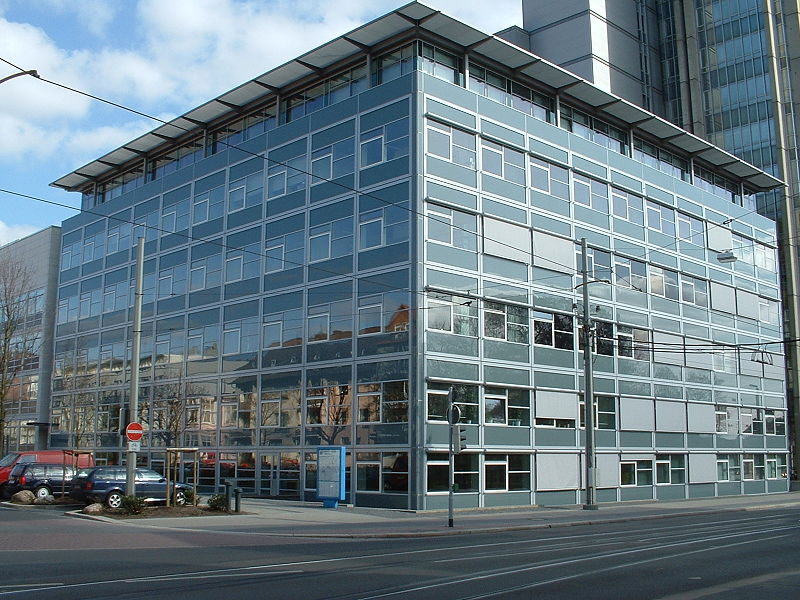
\includegraphics{infozentrum}
\end{gaussbox}
%
\begin{gaussbox}[bgcolor=tubsGray20,padding=default]{1}{3}{2}{1}
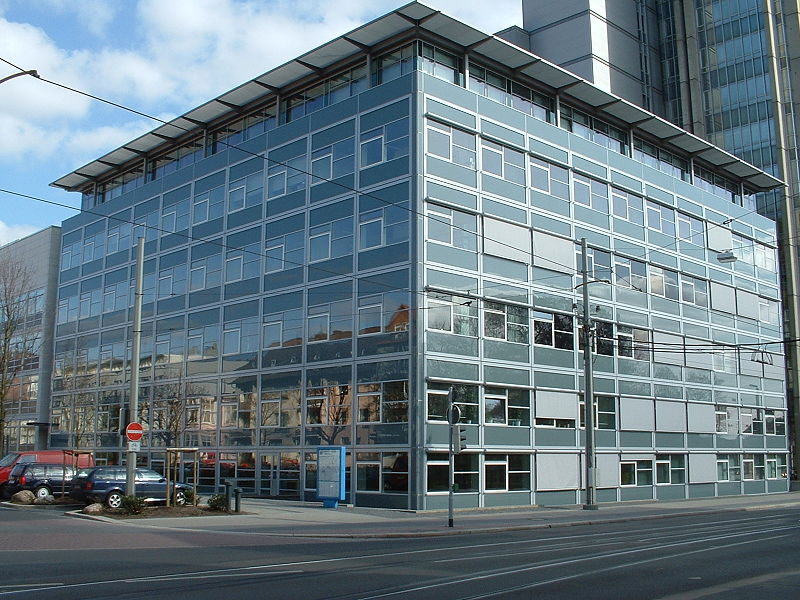
\includegraphics{infozentrum}
\end{gaussbox}
\begin{gaussbox}[bgcolor=tubsGray20,padding=none]{3}{3}{2}{1}
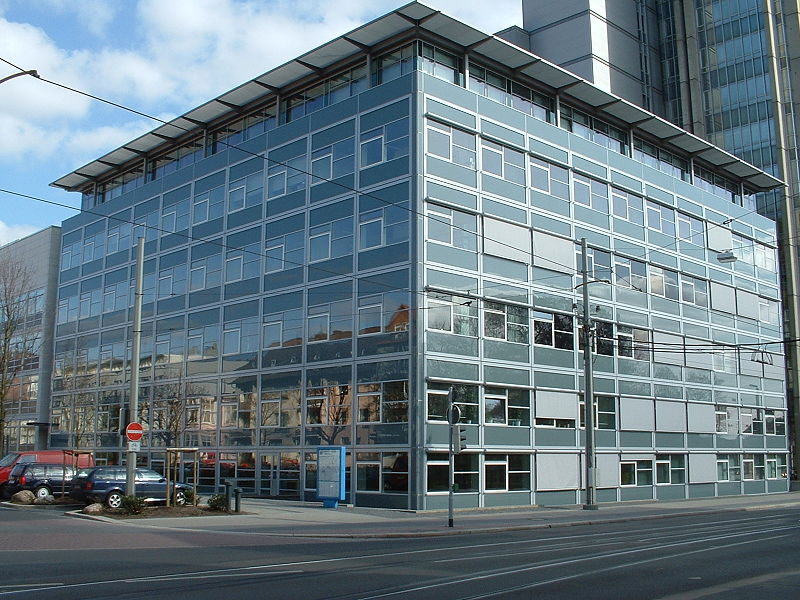
\includegraphics{infozentrum}
\end{gaussbox}
\begin{gaussbox}[bgcolor=tubsBlue20,padding=minimal]{5}{3}{2}{1}
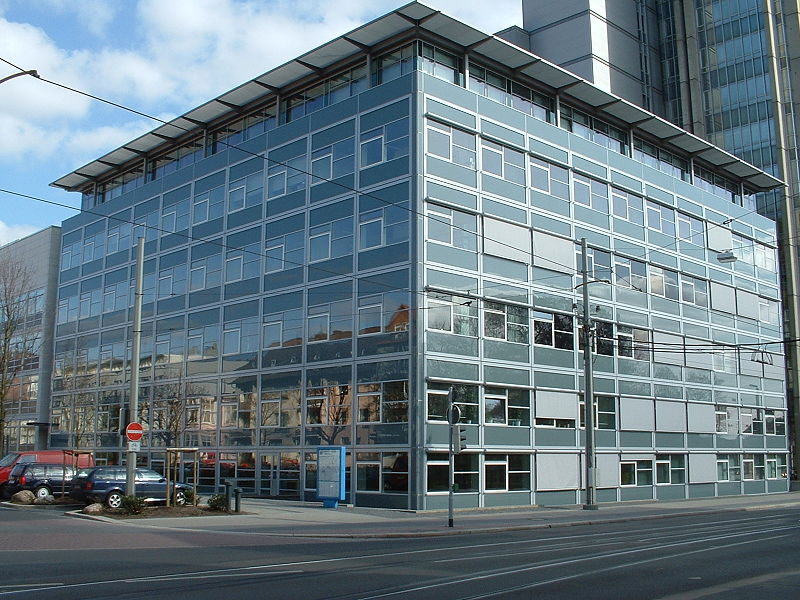
\includegraphics{infozentrum}
\end{gaussbox}
%
% \begin{gaussbox}[bgcolor=tubsGray20]{2}{4}{5}{2}
% \end{gaussbox}
\begin{gaussbox}[fgcolor=tuRed]{2}{4}{5}{2}
\raggedright\sffamily
\lipsum[1]
\end{gaussbox}
\clearpage


\end{document}
